\chapter{REMD: GPU ACCELERATION AND EXCHANGES IN MULTIPLE DIMENSIONS}
\label{ch5}

This chapter contains a description of my work implementing replica exchange
molecular dynamics (REMD) in the \emph{pmemd} program of the Amber program
suite. \cite{AMBER12}. The first sections describe the general theory of the
state exchanges supported by Amber, followed by details of their implementation.
I then describe my design of multiple-dimension REMD in Amber and provide some
sample studies performed using the code.

\section{Temperature REMD}

The most common variant of REMD simulations involves assigning replicas with
different temperatures (T-REMD). \cite{Sugita_ChemPhysLett_1999_v314_p141} In
typical T-REMD simulations, the Monte Carlo-based replica exchange attempts
occur between a pair of replicas at different temperatures. The exchange success
probability---calculated in a way that satisfies detailed balance to preserve
valid thermodynamics---is solved for the proposed change of two replicas
swapping temperatures, as shown in Eq. \ref{eq5:TExchProb}.  When $2N$ replicas
are present, $N$ independent exchange attempts can be made simultaneously
between different pairs of replicas. If no replica is involved in multiple
exchange attempts, these moves can be evaluated independently. While this may
not be the most efficient way to perform replica exchange attempts, it is the
most common approach due to its simplicity and efficiency.

To calculate the exchange probability in T-REMD exchange attempts, we start with
the detailed balance equation (Eq. \ref{eq1:DetailedBalance}) in which replicas
$m$ and $n$ have temperatures $T_m$ and $T_n$, respectively in our initial state
$i$. The temperatures swap in our proposed state such that replicas $m$ and $n$
have temperatures $T_n$ and $T_m$, respectively. Because the potential energy
function of each replica is the same---only the temperature differs between
replicas---the probability of a replica having a specific temperature is
directly proportional to the Boltzmann factor (in the canonical ensemble). The
derivation of the exchange probability equation in T-REMD simulations is shown
in Eq. \ref{eq5:TExchProb}.

\begin{align}
   P_{i} \pi_{i \rightarrow j} & = P_{j} \pi_{j \rightarrow i} \nonumber \\
   \frac {\exp \left[ -\beta_m E_m \right] \exp \left[ -\beta_n E_n \right]}
         {Q_m Q_n} \pi_{i \rightarrow j} & = \frac {\exp \left[ -\beta_n E_m
         \right] \exp \left[ -\beta_m E_n \right]} {Q_n Q_m} \pi_{j \rightarrow
         i} \nonumber \\
%  \exp \left[ -\beta_m E_m - \beta_n E_n \right] \pi_{i \rightarrow j} & =
%        \exp \left[ -\beta_n E_m - \beta_m E_n \right] \pi_{j \rightarrow i}
%        \nonumber \\
%  \frac {\pi_{i \rightarrow j}} {\pi_{j \rightarrow i}} & = \frac {\exp \left[
%        -\beta_n E_m - \beta_m E_n \right]} {\exp \left[ -\beta_m E_m - \beta_n
%        E_n \right]} \nonumber \\
%  \frac {\pi_{i \rightarrow j}} {\pi_{j \rightarrow i}} & = \exp \left[
%        -\beta_n E_m - \beta_m E_n + \beta_m E_m + \beta_n E_n \right]
%        \nonumber \\
   \frac {\pi_{i \rightarrow j}} {\pi_{j \rightarrow i}} & = \min \left \lbrace
         1, \exp \left[ (\beta_n - \beta_m) (E_n - E_m) \right] \right \rbrace
   \label{eq5:TExchProb}
\end{align}
where $\beta_m$ is $1/k_BT_m$ for replica $m$ and $E_m$ is the potential energy
of the structure in replica $m$.

Because the temperature of the system uniquely defines its kinetic energy, the
potential energy can be used in lieu of the total energy in Eq.
\ref{eq5:TExchProb} as long as the total temperature remains consistent after
the exchange attempt completes. Therefore, the momenta of replica $m$ are
typically scaled by $\sqrt{T_n/T_m}$ after successfully exchanging with replica
$n$. \cite{Sugita_ChemPhysLett_1999_v314_p141} By scaling the velocities in this
way, snapshots following a successful exchange attempt are immediately
`equilibrated' members of the new temperature's ensemble, thereby eliminating
the need to relax the structure to its `new' temperature. This allows REMD
simulations to be carried out more efficiently by permitting exchange attempts
very frequently. \cite{Sindhikara2008, Sindhikara2010}

An important consideration for T-REMD simulations is how many temperature
replicas you should use as well as what temperatures those replicas should have.
As the temperature of a system increases, the number of low-energy structures
that are sampled during the simulation decreases. In fact, at infinite
temperatures, MD is effectively equivalent to random sampling, whose
consequences are illustrated in Fig. \ref{fig1:EthanMC}. The temperature ladder
(\ie the selection of temperatures at which to run each replica) should be
chosen so as to optimize the simulation efficiency. If the temperature
difference between adjacent replicas is too great, then the average potential
energy difference between adjacent replicas will be large and the exchange
probability in Eq. \ref{eq5:TExchProb} will be very small. As a result, the low
temperature ensembles will not benefit from the enhanced sampling achievable at
the higher temperatures. On the other hand, if the temperature difference
between adjacent replicas is too small, then computational effort will be wasted
by simulating unnecessary replicas that do not enhance sampling from the
generalized ensemble.

By analyzing Eq. \ref{eq5:TExchProb}, it is clear that in order to have a high
exchange acceptance probability, either the temperature difference or the
potential energy difference between exchanging replicas must be small---in the
extreme case, if a higher temperature replica has a conformation whose potential
energy is less than or equal to the lower-temperature replica, that exchange
attempt is always accepted. By plotting the potential energy distributions
obtained from a short simulation at each temperature, the exchange rate between
any two replicas can be estimated based on the degree by which their potential
energy distributions overlap, shown in Fig. \ref{fig5:TempOverlap}. A good
choice of temperatures for each replica can be made \emph{a priori} based simply
on the number of degrees of freedom present in the system.
\cite{TREMD_Predictor} 

\begin{figure}
   \includegraphics[width=6.5in]{TempOverlap.ps}
   \caption{Potential energy distributions of TrpCage---a 20-residue
            peptide---at various temperatures in a T-REMD simulation.}
   \label{fig5:TempOverlap}
\end{figure}

One challenge with T-REMD is its scalability for large systems. It is well-known
that thermodynamic fluctuations scale as $1/\sqrt{N}$ in statistical ensembles
where $N$ is the total particle count. Therefore, the larger a system gets, the
narrower its potential energy distribution becomes. Consequently, as the
potential energy distributions narrow, replicas must be spaced closer and closer
together to achieve sufficient mixing along the temperature-space parameter. For
this reason, T-REMD simulations on systems that are explicitly solvated are
rare. While some approaches, like the one by \citeauthor{Okur2006}, use a hybrid
solvation scheme whereby exchange attempts are carried out in implicit solvent,
the first two solvation layers are often represented poorly by implicit solvent,
requiring their inclusion even in the hybrid approach. \cite{Okur2006}

Furthermore, the snapshots generated at higher temperatures in the generalized
ensemble are typically discarded from analyses for two reasons. First, we are
typically interested in the thermodynamics of room temperature, so the
high-temperature dynamics are not of general interest. Second, our force fields
are parametrized for use at temperatures near \mbox{300 K}, and higher
temperatures may break the applicability of harmonic functions for several
bonded potentials. While the high-temperature data may be reweighted for
inclusion in low-temperature ensembles,
\cite{Chodera_JChemTheoryComput_2007_v3_p26} higher temperature replicas
contribute increasingly little information to the temperatures of interest.

\section{Hamiltonian REMD}

Another common variant of REMD simulations involves swapping Hamiltonians
between replicas (H-REMD). Because the nature of the exchange in H-REMD
simulations is fundamentally different from those in T-REMD, Eq.
\ref{eq5:TExchProb} cannot be used to calculate the exchange probability for
H-REMD simulations. The proper exchange probability for H-REMD simulations,
generalized for running replicas at different temperatures, is derived in Eq.
\ref{eq5:HExchProb}. Eq. \ref{eq5:HExchProbNotemp} is the special case of Eq.
\ref{eq5:HExchProb} when the temperatures of exchanging replicas is the same.
The easiest and most general way of implementing H-REMD is to swap coordinates
between exchanging replicas. This approach, as implemented in Amber, can be used
for umbrella sampling REMD, \cite{Babin_JChemPhys_2008_v128_p134101,
Sugita_JChemPhys_2000_v113_p6042} accelerated REMD with different boost
parameters, \cite{Fajer_JComputChem_2009_v30_p1719,
Arrar_JChemTheoryComput_2013_v9_p18} and alchemical changes between two end
states. \cite{Meng_JChemTheoryComput_2011_v7_p2721} As a result, Eq.
\ref{eq5:HExchProb} is derived subject exchanging coordinates only.

\begin{align}
   P_{i} \pi_{i \rightarrow j} & = P_{j} \pi_{j \rightarrow i} \nonumber \\
   \frac {\exp \left[ -\beta_m H_m(\vec{x}_m) \right] \exp \left[ -\beta_n
         H_n(\vec{x}_n) \right]} {Q_m Q_n} \pi_{i \rightarrow j} & = \frac {\exp
         \left[ -\beta_m H_m(\vec{x}_n) \right] \exp \left[ -\beta_n
         H_n(\vec{x}_m) \right]} {Q_n Q_m} \pi_{j \rightarrow i} \nonumber \\
%  \exp \left[ -\beta_m E_m - \beta_n E_n \right] \pi_{i \rightarrow j} & =
%        \exp \left[ -\beta_n E_m - \beta_m E_n \right] \pi_{j \rightarrow i}
%        \nonumber \\
%  \frac {\pi_{i \rightarrow j}} {\pi_{j \rightarrow i}} & = \frac {\exp \left[
%        -\beta_n E_m - \beta_m E_n \right]} {\exp \left[ -\beta_m E_m - \beta_n
%        E_n \right]} \nonumber \\
%  \frac {\pi_{i \rightarrow j}} {\pi_{j \rightarrow i}} & = \exp \left[
%        -\beta_n E_m - \beta_m E_n + \beta_m E_m + \beta_n E_n \right]
%        \nonumber \\
   \frac {\pi_{i \rightarrow j}} {\pi_{j \rightarrow i}} & = \min \left \lbrace
         1, \exp \left[ (\beta_n - \beta_m) (E_n - E_m) \right] \right \rbrace
\end{align}

\section{Multi-Dimensional REMD}

\section{Implementation}

\subsection{GPU Acceleration}

\subsection{MPI Communicator Topology}
